\documentclass[journal,12pt,onecolumn]{IEEEtran}
\usepackage[utf8]{inputenc}   % Codificación de entrada
\usepackage[T1]{fontenc}      % Codificación de fuente
\usepackage[spanish,es-tabla]{babel}   % Idioma español
\usepackage{lmodern}          % Fuente moderna
\usepackage{amsmath, amssymb} % Matemáticas y símbolos
\usepackage{graphicx} 		  % Gráficos e imágenes
\graphicspath{{img/}{tablas/}{portada/}}  % Las imágenes se buscarán en la carpeta "img"
\usepackage{longtable}      % Para tablas que se extienden en varias páginas
\usepackage{tabularx}	% Tablas avanzadas
\usepackage{threeparttable}
\usepackage{hyperref}	% Hipervínculos

%-------------------------------------------
% Otros paquetes útiles (personaliza según tus necesidades)
%-------------------------------------------
\usepackage{caption}
\usepackage{subcaption}
\usepackage{xcolor}
\usepackage{setspace}

%-------------------------------------------
% Comandos personalizados
\renewcommand{\listtablename}{Índice de tablas}
\renewcommand{\appendixname}{Anexos}
\definecolor{colorreferences}{RGB}{48,134,3}

% Metadatos del PDF
\hypersetup{
	unicode=true,
	hidelinks,
	colorlinks=true,       % false: boxed links; true: colored links
	linkcolor=black,          % color of internal links (change box color with linkbordercolor)
	citecolor=colorreferences,        % color of links to bibliography
	filecolor=magenta,      % color of file links
	urlcolor=blue,           % color of external links
	linkbordercolor={0 0 0}
}
%-------------------------------------------
% Inicio del documento
%-------------------------------------------
\begin{document}

% Aquí se encuentra el archivo con la portada
\begin{titlepage}
	\centering
	%-------------------------------------------
	% Logos en una tabla: izquierda, centro y derecha
	\begin{tabular}{@{}p{0.3\textwidth} p{0.3\textwidth} p{0.3\textwidth}@{}}
		
\includegraphics[height=2cm]{tecnm} & 
		\centering 
\includegraphics[height=1.5cm]{SEP} & 
		\raggedleft 
\includegraphics[height=2cm]{ith.jpg} \\
	\end{tabular}
	
	\vspace{2em}
	
	\noindent
	%-------------------------------------------
	%	Información institucional y académica (esquina superior izquierda)
	\begin{minipage}[t]{0.48\textwidth}
		\raggedright
		\small \textbf{%
			Instituto Tecnológico de Hermosillo\\
			Materia: Robótica\\
			Profesor: Medina Gil Lamadrid, Jesús Iván%
		}
	\end{minipage}%
	\hfill
	%	fecha actual (esquina superior derecha), en letras pequeñas y en negrita.
	\begin{minipage}[t]{0.48\textwidth}
		\raggedleft
		\small \textbf{\today}
	\end{minipage}
	
	\vspace{2em}
	
	%-----------------------------------------
	% Unidad y Título de la tarea en letras grandes y en negrita
	{\large \textbf{Unidad 1: Morfología del robot}}\\
	{\Huge \textbf{Tipos de Sensores}}
		
	\vspace{1em}
	
	%---------------------------------------
	% Tabla con la información del equipo
	%---------------------------------------
	% Encabezado del equipo
	\begin{center}
		{\Large \textbf{Equipo 2}}
	\end{center}
	
	\vspace{1em}
	
	% Tabla de integrantes:
	% Cada fila contiene: foto (columna izquierda) y datos del integrante (columna derecha)
	\begin{center}
		\begin{tabular}{c c}
			\begin{tabular}{c}
				
\includegraphics[height=3cm]{Cedano.jpeg} \\
				\textbf{Cedano Mendoza},\\ Carlos Francisco \\ \texttt{L21330552@hermosillo.tecnm.mx} \\ Teléfono: 6624686707
			\end{tabular} &
			\begin{tabular}{c}
				
\includegraphics[height=3cm]{Martinez.png} \\
				\textbf{Martinez Navarro,}\\ Sebastian \\ \texttt{L2133} \\ Teléfono: 6621053764
			\end{tabular} \\ \vspace{2em}
			\begin{tabular}{c}
				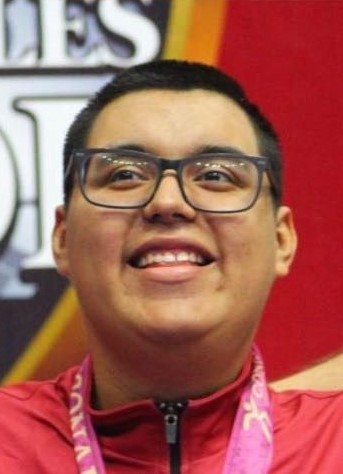
\includegraphics[height=3cm]{Ocampo.jpeg} \\
				\textbf{Ocampo Ramos,}\\ Addiel Adrián \\ \texttt{L20330895@hermosillo.tecnm.mx} \\ Teléfono: 6623501716
			\end{tabular} &
			\begin{tabular}{c}
				\includegraphics[height=3cm]{Pérez.jpeg} \\
				\textbf{Pérez Estupiñán,}\\ Ana Claudia \\ \texttt{L21330669@hermosillo.tecnm.mx} \\ Teléfono: 6624281154
			\end{tabular}
		\end{tabular}
	\end{center}

\end{titlepage}

%	Es innecesario poner el índice porque ya aparece en los marcadores del PDF
%\tableofcontents

% Ejemplo de inclusión de una sección (por ejemplo, "introduccion.tex" debe estar en la carpeta "secciones" y se recomienda no usar carácteres especiales (tilde) o espacios)
\section{Robot Ejemplo}

	\begin{figure}[h]
	\centering
	\subfloat[Figura de Matlab robot ejemplo.]{%
		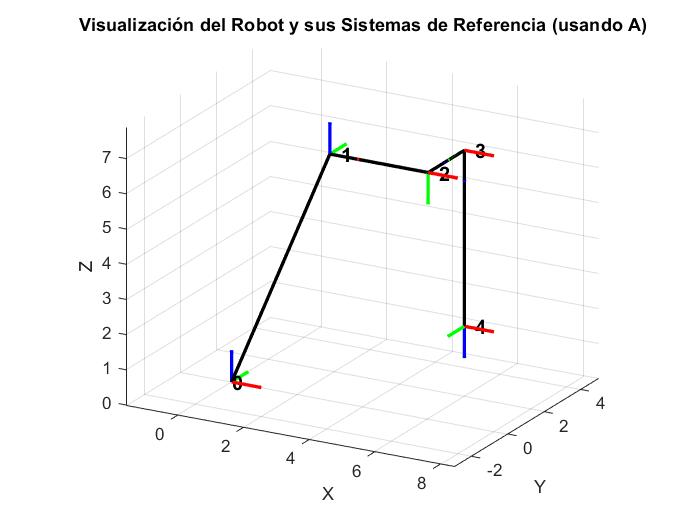
\includegraphics[width=0.47\textwidth]{ROBOTEJEMPLOMATLAB.jpg}%
		
	}
	\hspace{0.5cm} % Espacio entre imágenes (ajusta el valor si es necesario)
	\subfloat[Diagrama de lineas robot ejemplo.]{%
		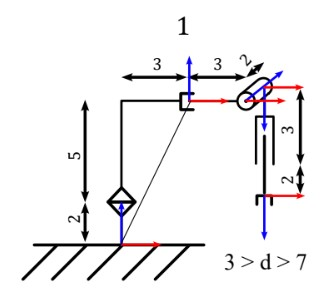
\includegraphics[width=0.45\textwidth]{DIAGRAMAROBOTEJEMPLO.jpg}%
		
	}
	\caption{Ejemplo de Denavit Hartenberg.}
	
\end{figure}
\section{Robot 4}

	\begin{figure}[h]
	\centering
	\subfloat[Figura de Matlab Robot 4.]{%
		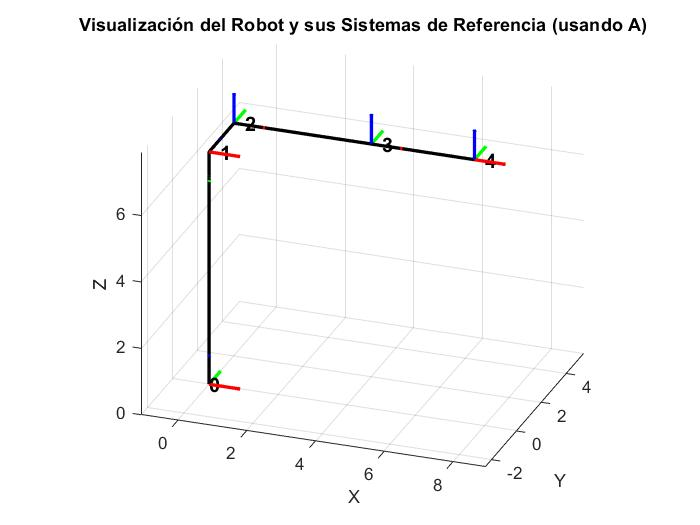
\includegraphics[width=0.5\textwidth]{ROBOT4MATLAB.jpg}%
		
	}
	\hspace{0.5cm} % Espacio entre imágenes (ajusta el valor si es necesario)
	\subfloat[Diagrama de lineas Robot 4.]{%
		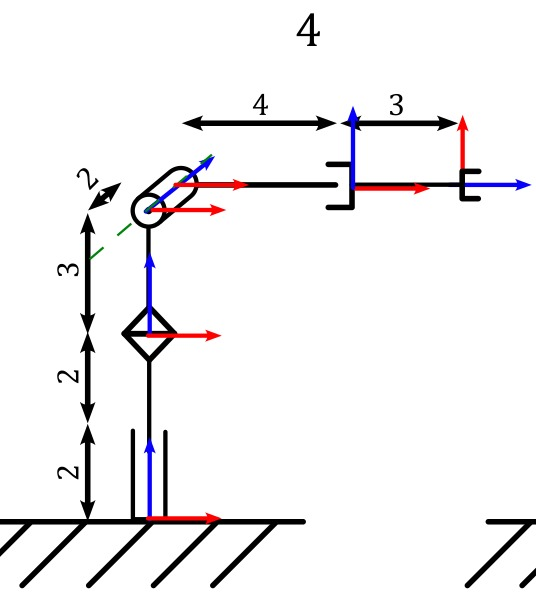
\includegraphics[width=0.35\textwidth]{DIAGRAMAROBOT4.jpeg}%
		
	}
	\caption{Ejercicio 4 de Denavit Hartenberg.}
	
\end{figure}
\vspace{8cm}
\section{Robot 5}

	\begin{figure}[h]
	\centering
	\subfloat[Figura de Matlab Robot 5.]{%
		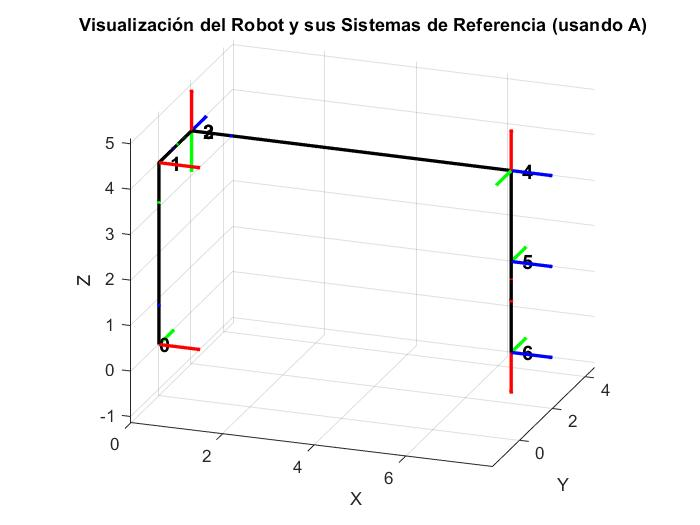
\includegraphics[width=0.45\textwidth]{ROBOT5MATLAB.jpg}%
		
	}
	\hspace{0.5cm} % Espacio entre imágenes (ajusta el valor si es necesario)
	\subfloat[Diagrama de lineas Robot 5.]{%
		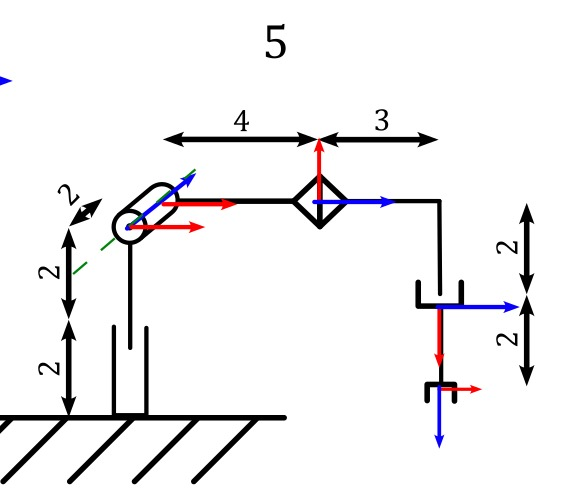
\includegraphics[width=0.45\textwidth]{DIAGRAMAROBOT5.jpeg}%
		
	}
	\caption{Ejercicio 5 de Denavit Hartenberg.}
	
\end{figure}
\vspace{1cm}
\section{Robot 6}

	\begin{figure}[h]
	\centering
	\subfloat[Figura de Matlab Robot 6.]{%
		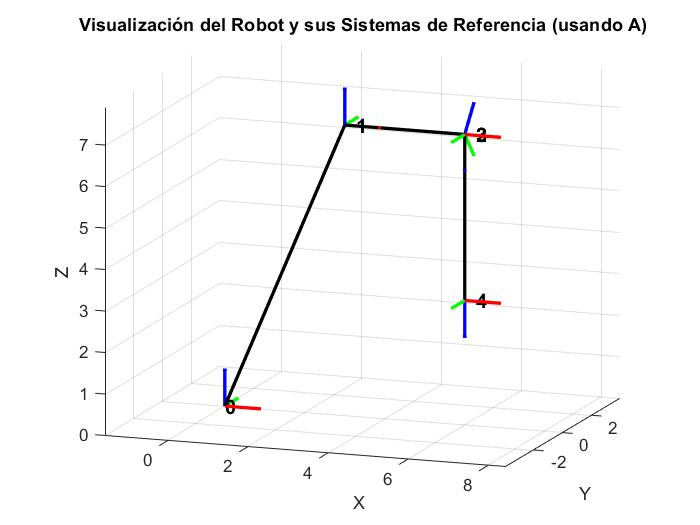
\includegraphics[width=0.45\textwidth]{ROBOT6MATLAB.jpg}%
		
	}
	\hspace{0.5cm} % Espacio entre imágenes (ajusta el valor si es necesario)
	\subfloat[Diagrama de lineas Robot 6.]{%
		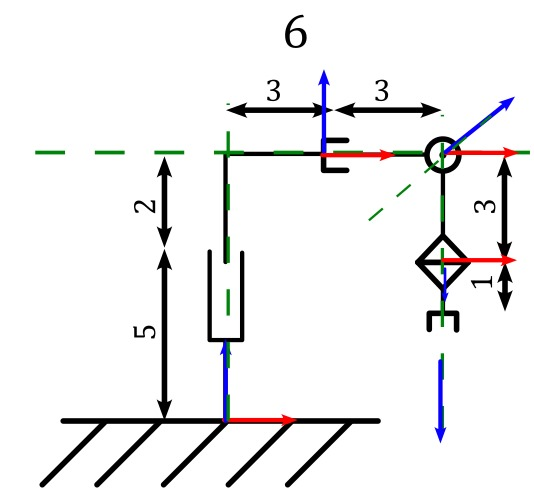
\includegraphics[width=0.45\textwidth]{DIAGRAMAROBOT6.jpeg}%
		
	}
	\caption{Ejercicio 6 de Denavit Hartenberg.}

\end{figure}
\vspace{3cm}
\section{Robot 7}

	\begin{figure}[h]
	\centering
	\subfloat[Figura de Matlab Robot 7.]{%
		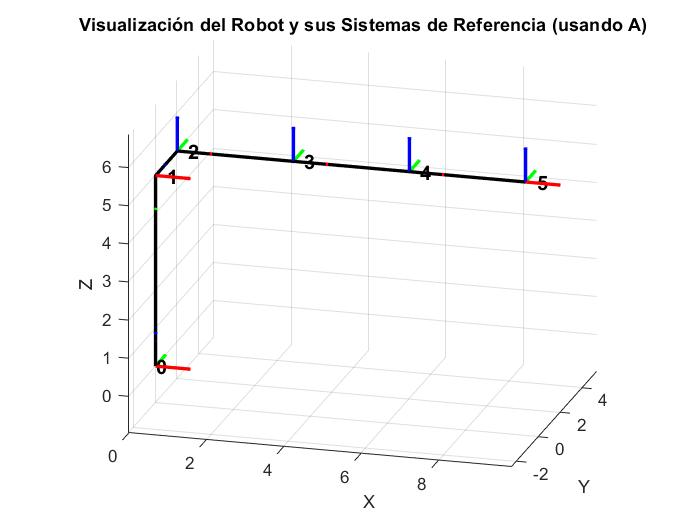
\includegraphics[width=0.45\textwidth]{ROBOT7MATLAB.jpg}%
	
	}
	\hspace{0.5cm} % Espacio entre imágenes (ajusta el valor si es necesario)
	\subfloat[Diagrama de lineas Robot 7.]{%
		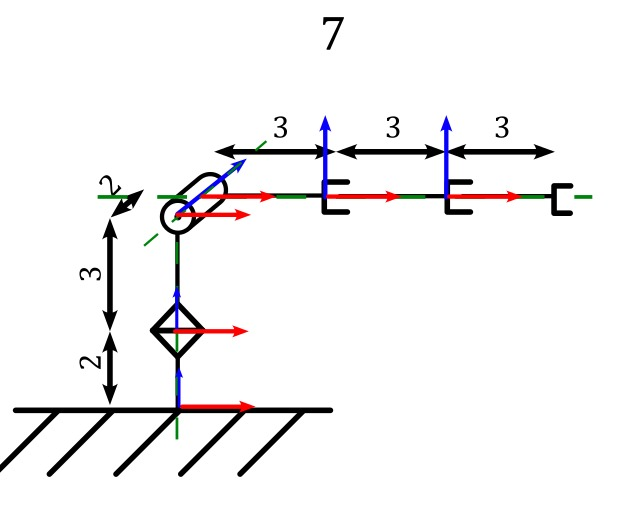
\includegraphics[width=0.45\textwidth]{DIAGRAMAROBOT7.jpeg}%
		
	}
	\caption{Ejercicio 7 de Denavit Hartenberg.}

\end{figure}
\section{Robot 8}

	\begin{figure}[h]
	\centering
	\subfloat[Figura de Matlab Robot 8.]{%
		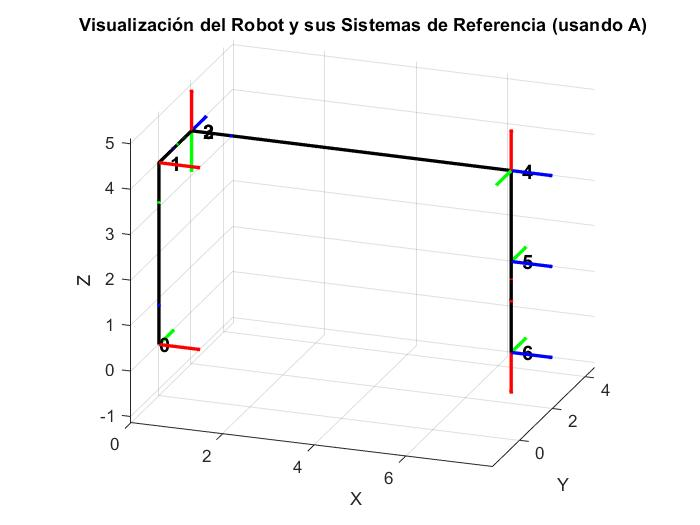
\includegraphics[width=0.45\textwidth]{ROBOT5MATLAB.jpg}%
	}
	\hspace{0.5cm} % Espacio entre imágenes (ajusta el valor si es necesario)
	\subfloat[Diagrama de lineas Robot 8.]{%
		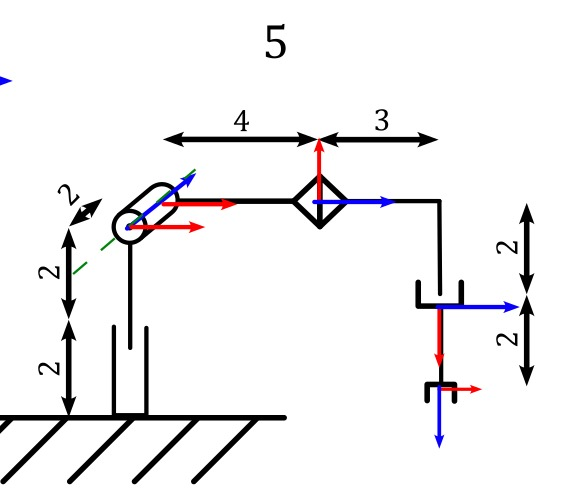
\includegraphics[width=0.45\textwidth]{DIAGRAMAROBOT5.jpeg}%
	}
	\caption{Ejercicio 5 de Denavit Hartenberg.}
\end{figure}

%-------------------------------------------
% Bibliografía
%-------------------------------------------
\bibliographystyle{IEEEtran}  % Estilo de bibliografía IEEE
% La bibliografía se tomará del archivo "fuentes.bib"
%\bibliography{fuentes}
	
\end{document}
